\section{Recursive neural network models} \label{methods}

The models that we study are are centered aronund a recursively applied composition function which is meant to mimic the recursive construction of meanings in formal semantics. In this scheme, pairs of words are merged into phrase representations by a function that maps from representations of length $2N$ to representations of length $N$. These phrase representations are then further merged with other words and phrases until the entire phrase or sentence being evaluated is represented in a single vector. This vector is then used as the input to a classifier and used in a supervised learning task.

We use the model architecture proposed in \citet{bowman2013can} and depicted in Figure \ref{sample-figure}. The two phrases being compared are built up separately on each side of the tree using the same composition function until they have each been reduced to single vectors. Then, the two phrase vectors are fed into a separate comparison layer that is meant to generate a feature vector capturing the relation between the two phrases. The output of this layer is then given to a softmax classifier, which in turn produces a hypothesized distribution over the seven relations.

For a composition layer, we evaluate models with both the plain neural network layer function (eq. \ref{rnn}) and the RNTN layer function proposed in \citet{chen2013learning} (eq. \ref{rntn}). A sigmoid nonlinearity (elementwise $\tanh$) is applied to the output of either layer function, following Socher et al.
\begin{gather} \label{rnn}
y_{RNN} = f(\mathbf{M} [\vec{x}^{(l)}; \vec{x}^{(r)}] + b_i)\\ % TODO: Add column vectors?
\label{rntn}
y_{RNTN} = f(\vec{x}^{(l)T} \mathbf{A}^{[1...N]} \vec{x}^{(r)} + \mathbf{B} [\vec{x}^{(l)}; \vec{x}^{(r)}] + \vec{c})
\end{gather} % TODO: Explain third order tensor parameter?

The comparison layer uses the same type function template as the composition function (either an NN layer or an NTN layer) with independantly learned parameters and a separate nonlinearity function. Rather than use a $\tanh$ nonlinearity here, we found a substantial improvement in performance by using a rectified linear function for $f_{b}$. In particular, we use the leaky rectified linear function \cite{maasrectifier}: $f_{b}(\vec{x})=\max(\vec{x}, 0) + 0.01\min(\vec{x}, 0)$,  applied elementwise. 

To run the model forward and label a pair of phrases, the structure of the lower layers of the network is assembled so as to mirror the tree structures provided for each phrase. The word vectors are then looked up from the vocabulary matrix $V$ (one of the model parameters), and the composition and comparison functions are used to pass information up the tree and into the classifier at the top. For an objective function, we use the negative log of the probability assigned to the correct label.

We train the model with minibatch stochastic gradient descent (SGD) with learning rates computed using AdaGrad \cite{duchi2011adaptive} from a starting rate of 0.2. The parameters (including the vocabulary) are initialized randomly using a uniform distribution over $[-0.1, 0.1]$. % TODO: Update

\begin{figure}
\begin{center}
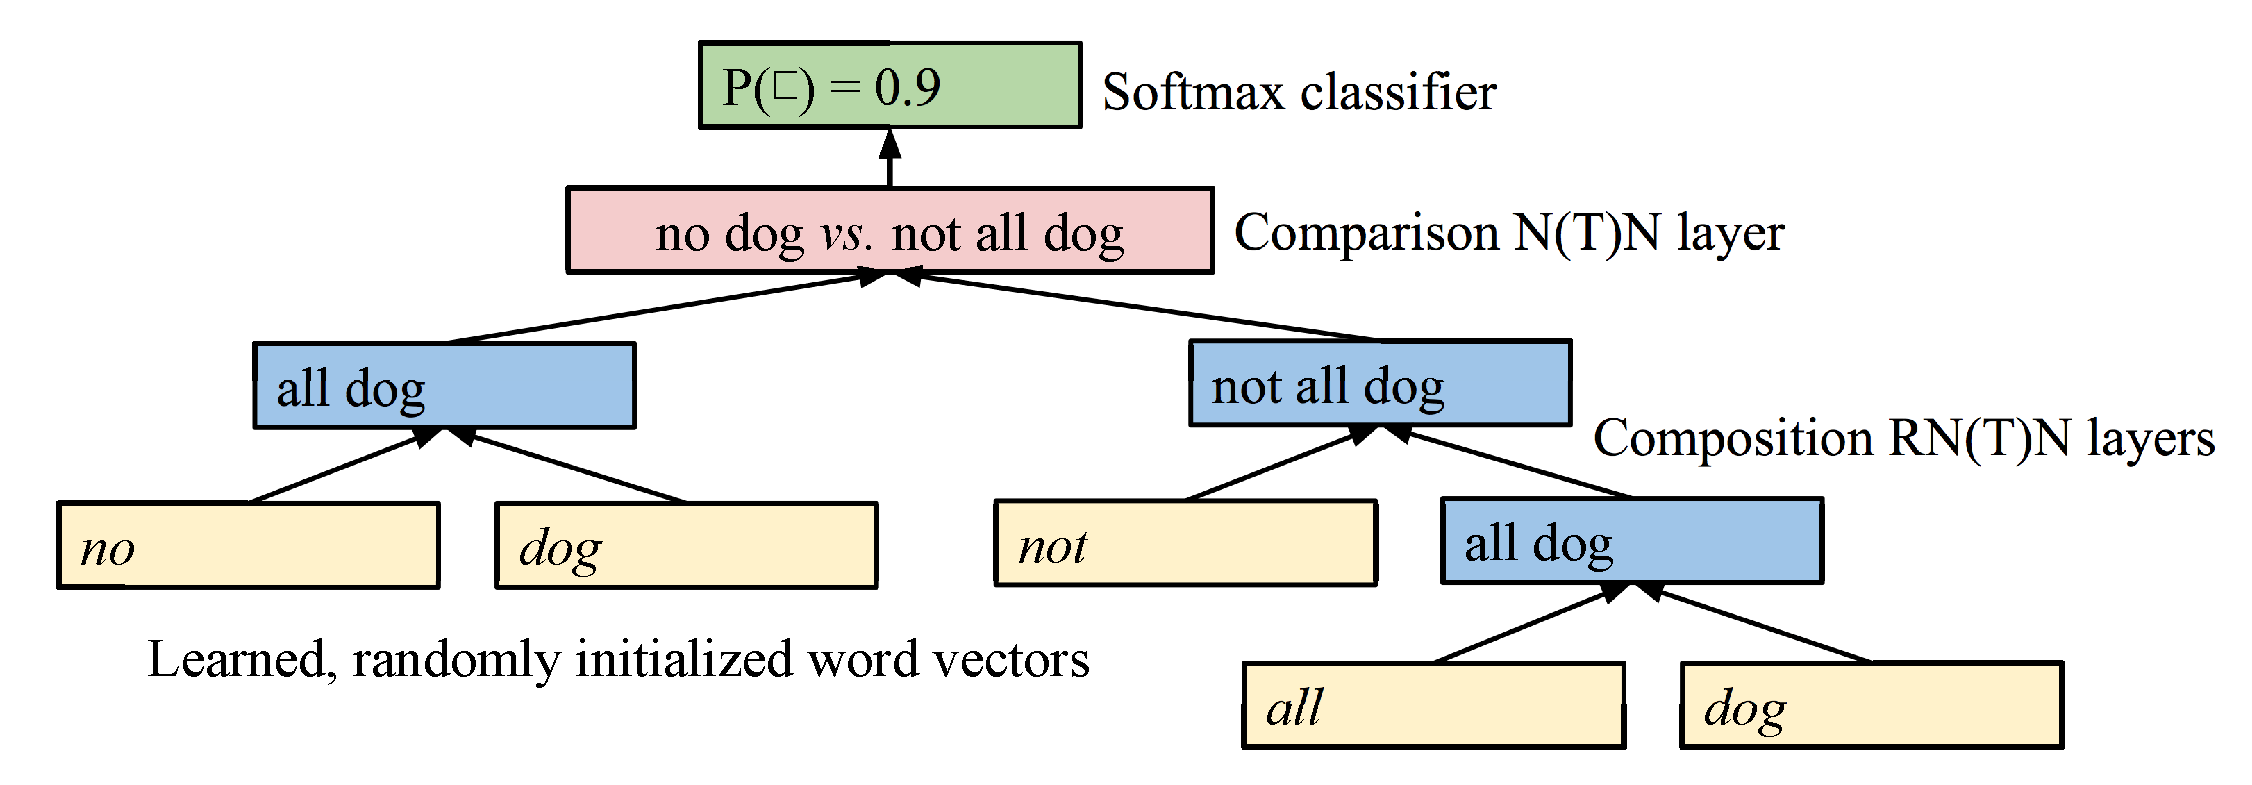
\includegraphics[scale=0.35]{model.eps}
\end{center}
\caption{The model structure used to compare \ii{no dog} and \ii{(not all) dog}. The same structure is used for both the RNN and RNTN layer functions. \label{sample-figure}} 
\end{figure}

\ii{Source code and generated data will be released after the conclusion of the review period.} % TODO: Or upon request? Attach anonymized code?
